
Nesse capítulo, será apresentado a construção do operador grosso Multiescala. A construção desse tipo de operador tem diversas aplicações para a solução dos sistemas lineares apresentados no capítulo \ref{ch:discretizacao}. Ele consiste basicamente em construir um operador grosso através do cálculo de funções de base em um grid gerado pelo acoplamento de elementos do grid fino. Pode ser utilizado como pré-condicionador \cite{casteletto}, como solver multinível semelhante aos solver multigrid ou ainda como aproximação para a solução original do problema. Os métodos multiescala tem sido aplicados com sucesso para problemas elípticos que é o caso do problema da elasticidade linear apresentado aqui. As vantagens do método apresentadas em \cite{thomashou} são que a funções de base multiescala tentam se adaptar as propriedades locais do operador de forma que o operador grosso as conserve, as funções de base podem ser construídas através da solução de problemas independentes e, portanto, em paralelo.

O primeiro passo para a construção do operador multiescala é gerar um novo grid com menos elementos que o grid original do problema (grid fino) que ainda representa o mesmo domínio $\Omega$. Esse grid novo será chamado de grid grosso e as variáveis relacionadas com ele serão assinadas com o sobre-escrito $H$. 
Assim grid grosso possui um conjunto $\tau_H$ de elementos onde cada elemento será uma aglomeração de elementos do grid fino. Por exemplo, a figura \ref{fig:gridgrosso} apresenta um grid grosso 3x3 construído a partir de um grid fino 7x7. É importante perceber que não existe a necessidade de aglomerar a mesma quantidade de elementos para se gerar o grid grosso já existem elementos formados por 9, 6 e 4 elementos do grid fino. Marcados de quadrados azuis estão mostrados os nós que pertencem ao grid grosso e grid fino.

\begin{figure}[!htbp]
\centering
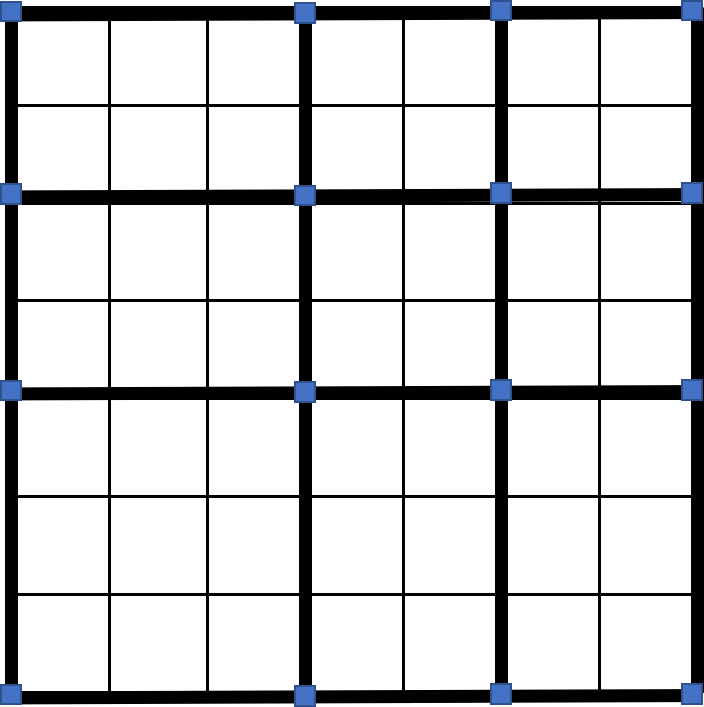
\includegraphics[width=6cm]{chap06/figs/grosso.png}
\caption{Exemplo de grid fino 7x7 e um grid grosso 3x3. O elemento inferior esquerdo é composto por 9 elementos do grid fino enquanto o elemento superior direito é composto com 4 elementos do grid fino.}
\label{fig:gridgrosso}

\end{figure}


No capítulo \ref{ch:discretizacao} foi apresentada a discretização através de elementos finitos para o problema de elasticidade linear através do método dos elementos finitos. A notação utilizada é baseada na utilizada em \cite{mbuck}. Assim, como naquele capítulo em que a função de desejada foi aproximada para um espaço $V^h$ formado por funções de base chapéu no domínio $\Omega$ do problema, a ideia agora é encontrar a solução do problema em um espaço grosso $V^{MS}$, tal que $V^{MS} \subset V^h$. 



Para definir melhor esse espaço $V^{MS}$ precisamos definir as suas funções de base geradoras. 


Novamente, para distinguir o nó pertencente ao grid grosso dos seus graus de liberdade o seguinte conjunto com graus de liberdade é criado.


\begin{equation}
    D^H = \{ p^{(m)} \in D^h : x^p \in \Sigma_H, m=1,2\}
\end{equation}



\section{Cálculo do NNZ do operador de Prolongamento}\label{sec:complexProlong}

Utilizar o método multiescala está associado a construção do operador grosso e também de levar os vetores entre o espaço fino e o grosso. Essas duas etapas necessitam de multiplicação pelos operadores $P$ e $P^T$. Essa seção visa tentar entender a complexidade dessas operações.

As dimensões do operador de prolongamento depende do número de graus de liberdade do operador fino e do operador grosso que é exatamente $\freedomfine \times \freedomcoarse$. Porém conforme visto no Capítulo \ref{ch:sistemas} a multiplicação de uma matriz esparsa por um vetor é da ordem de não zeros da matriz, assim apesar de um maior engrossamento do grid reduzir o valor de $n_u^H$ isso não necessariamente está associado a uma redução de não zeros de $P$.

Considerando um grid fino com $\numelementsxfine \times \numelementsyfine$ e um grid grosso onde cada elemento tem dimensões $q_x \times q_y$ e que mesmo os nós de fronteira com condição de contorno de Dirichlet não são removidos da matriz de rigidez, a quantidade de não zeros do operador de pronlogamento ($nnz_p$) pode ser calculada dividindo os nós em três conjuntos os nós interiores, nós vertice e os nós na aresta.  A Figura \ref{fig:gridCompleto} mostra cada um desse tipo de nós (em vermelho nó vértice, em azul nó aresta e em preto nó interior).


\begin{figure}[h]
\center
\subfigure[  ]{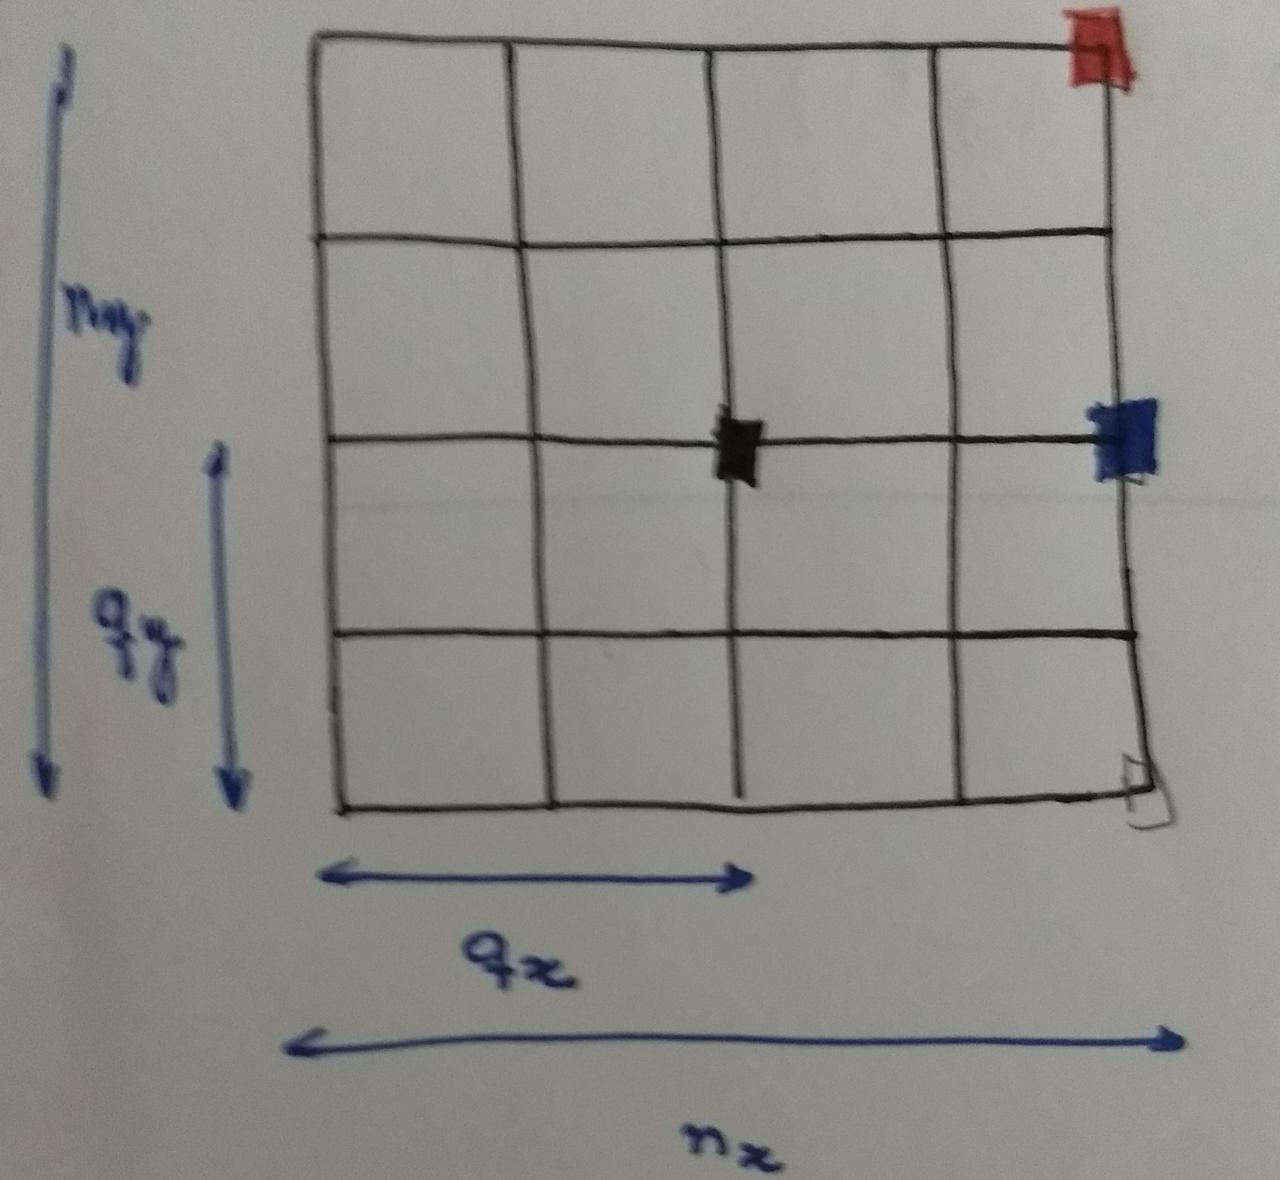
\includegraphics[width=0.45\textwidth]{chap06/figs/gridCompleto.jpeg}\label{fig:gridCompleto}}
\qquad
\subfigure[ ]{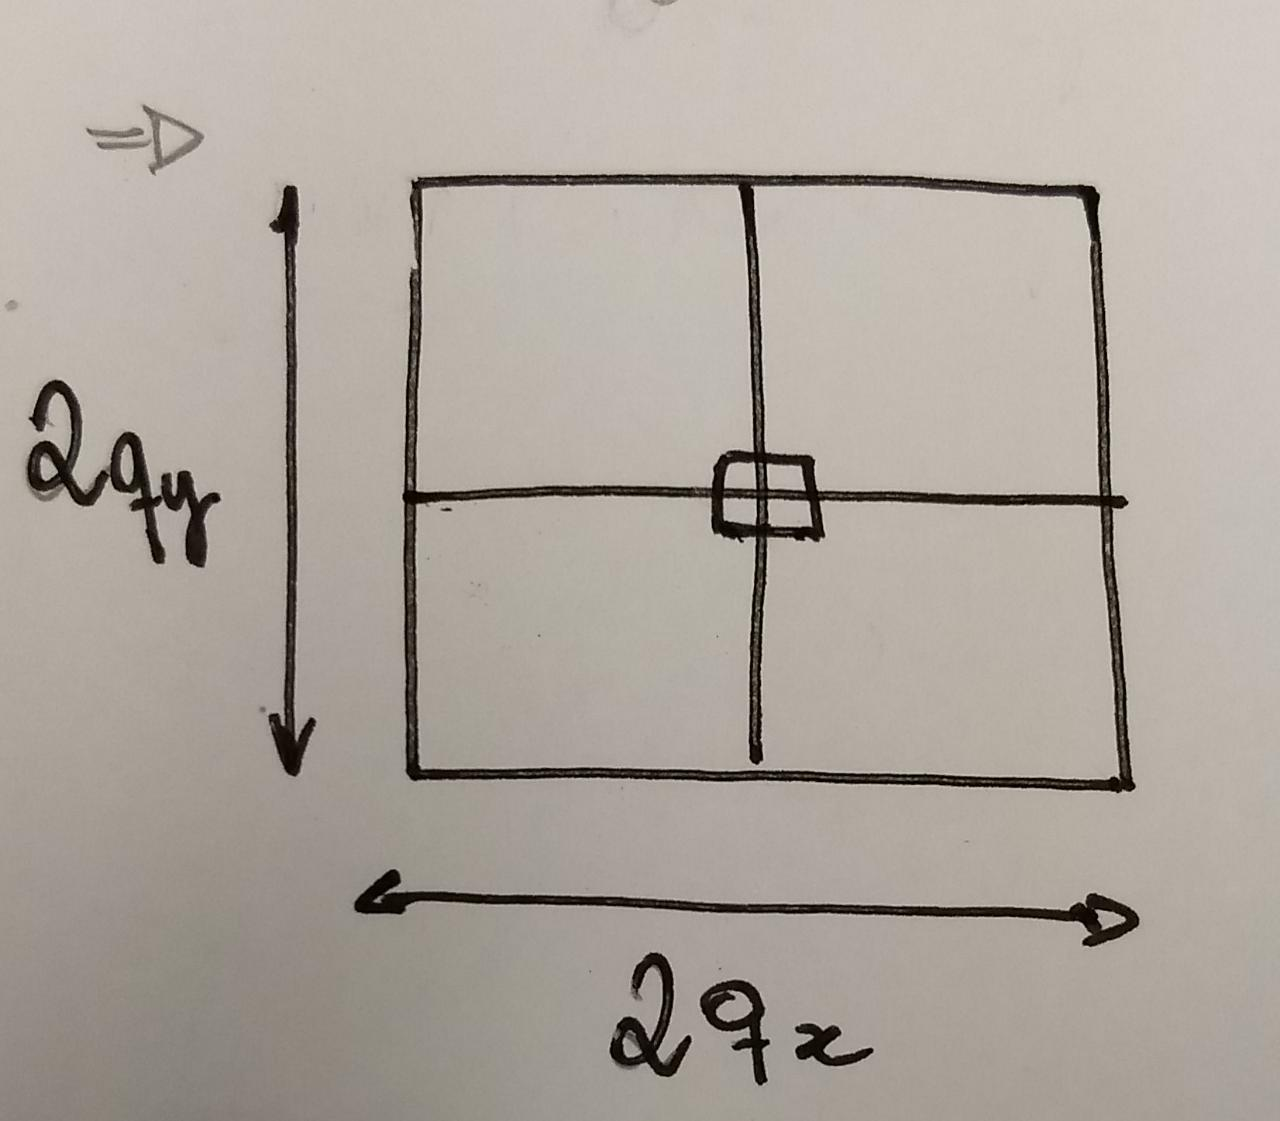
\includegraphics[width=0.45\textwidth]{chap06/figs/noInterior.jpeg}\label{fig:noInterior}}
\subfigure[ ]{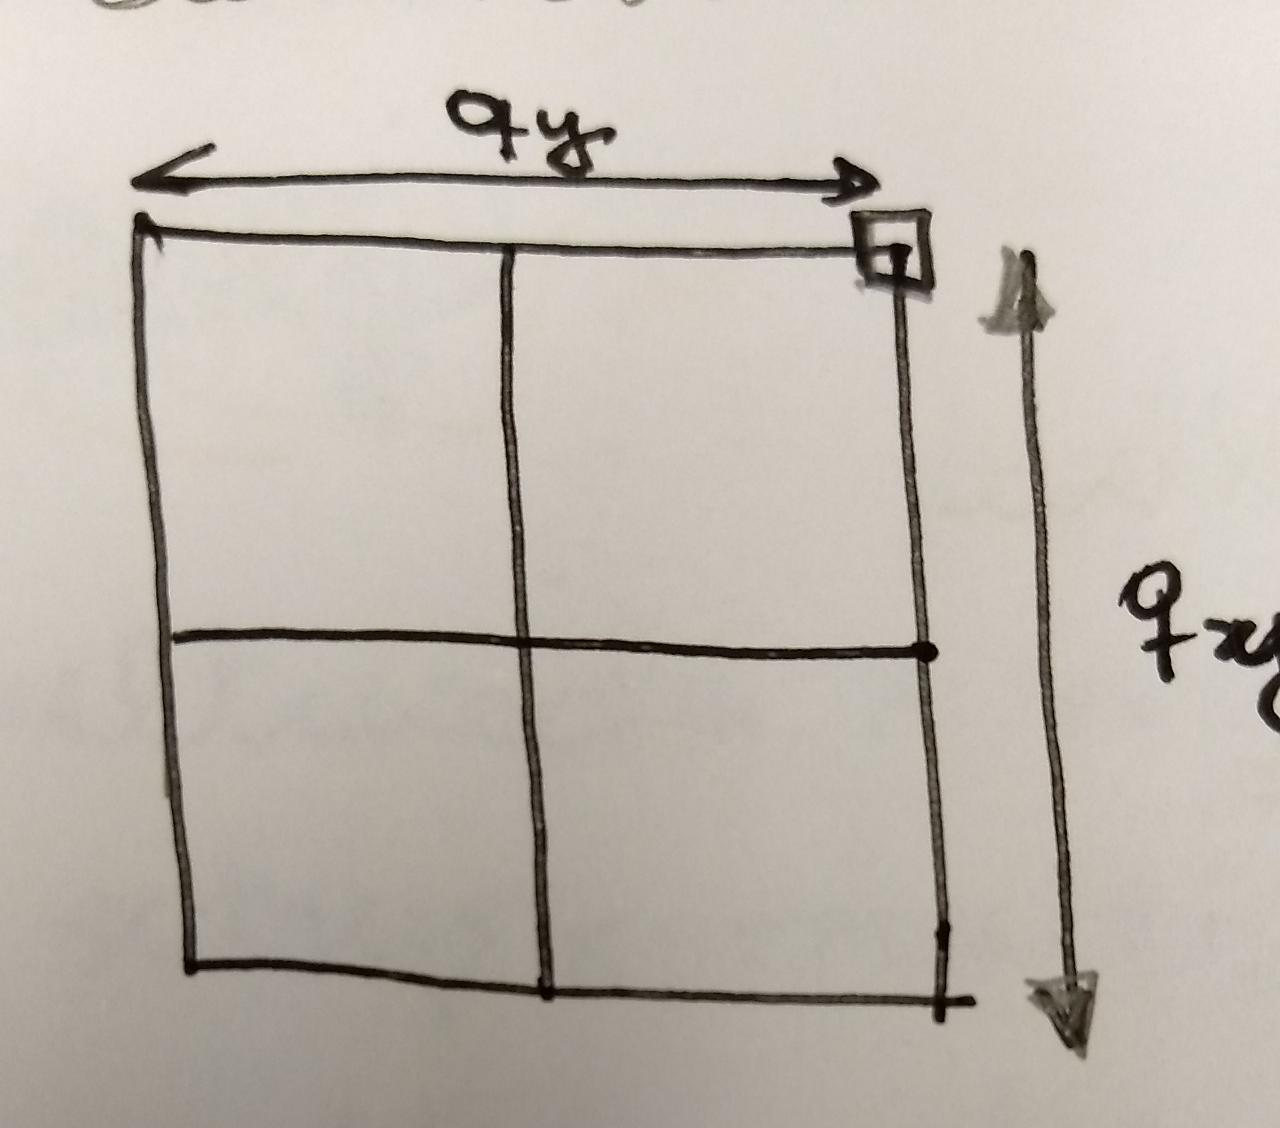
\includegraphics[width=0.45\textwidth]{chap06/figs/noVertice.jpeg}\label{fig:noVertice}}
\subfigure[ ]{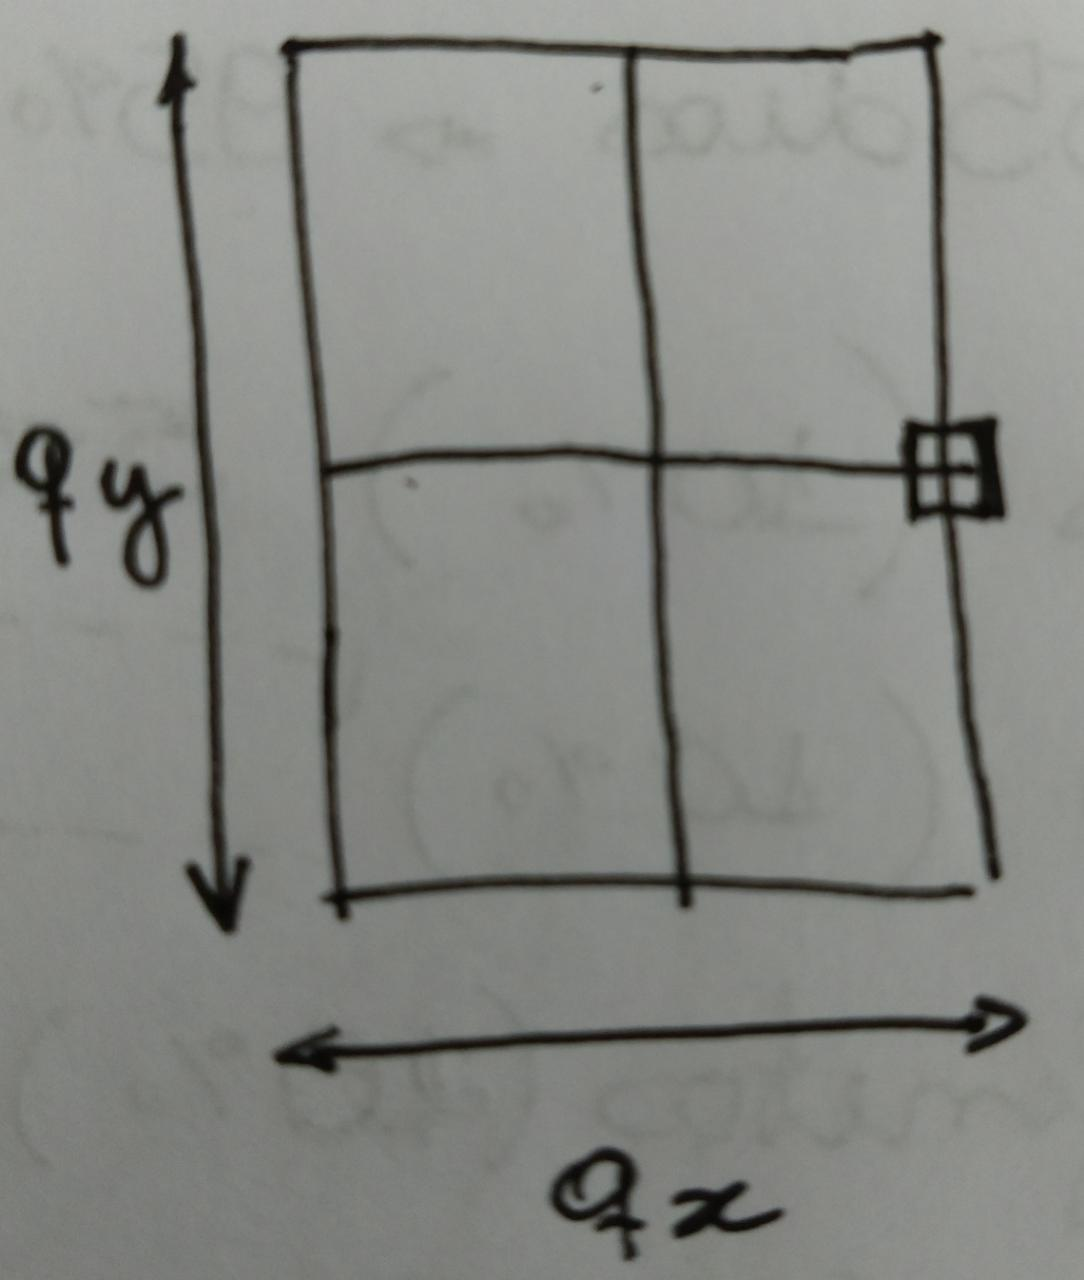
\includegraphics[width=0.45\textwidth]{chap06/figs/noAresta.jpeg}\label{fig:noAresta}}

\caption{Comparação da solução do grid fino com a solução do grid grosso.  }
\label{fig:verticesTypes}
\end{figure}

A quantidade de cada um desses nós na malha grossa é apresentado abaixo.

\begin{itemize}
    \item Nós interiores: $(\frac{n_x}{q_x} - 1) (\frac{n_y}{q_y} - 1)$
    \item Nós de aresta em $\Gamma_l$ e $\Gamma_r$: $2 ( \frac{n_y}{q_y} - 1)$
    \item Nós de aresta em $\Gamma_t$ e $\Gamma_b$: $2 ( \frac{n_x}{q_x} - 1)$
    \item Nós vértices: 4 
\end{itemize}


Cada nó tem duas funções de base associadas uma para cada grau de liberdade (x e y). Uma função de base de um vértice interior tem suporte em $(2q_x+1)(2q_y+1)$ outros nós como mostra a \ref{fig:noInterior}, além disso ela afeta os dois graus de liberdade de cada um desses nós, então cada um desses nós contribui com $4(2q_x+1)(2q_y+1)$ não zeros para o prolongamento (uma implementação mais cuidadosa do método pode economizar as bordas do suporte pois as funções se anulam). De maneira análoga, os nós vértices contribuem com $ 4 (q_x+1)(q_y+1)$, os nós aresta em $\Gamma_t$ e $\Gamma_b$ contribuem com $ 4 (2q_x+1)(q_y+1) $ e, finalmente, os nós arestas  $\Gamma_l$ e $\Gamma_r$ e contribuem com $ 4(q_x+1)(2q_y+1) $. Assim, para encontrar a quantidade total de não zeros do operador de prolongamento, basta multiplicar as quantidades de cada um dos nós pela duas contribuições conforme a Equação \eqref{eq:nnzRaw}. 


\begin{equation} \label{eq:nnzRaw}
\begin{aligned}
    nnz_P = & 4(2q_x+1)(2q_y+1)  (\frac{n_x}{q_x} - 1) (\frac{n_y}{q_y} - 1)   \\ 
            & + 4 (q_x+1)(2q_y+1)  2 ( \frac{n_y}{q_y} - 1) +  4 (2q_x+1)(q_y+1)  2 (\frac{n_x}{q_x} - 1) \\
            & +  4(q_x+1)(q_y+1) 4 
\end{aligned}
\end{equation}

Que pode ser modificada para a \eqref{eq:nnzRaw2},

\begin{equation} \label{eq:nnzRaw2}
\begin{aligned}
    nnz_P = &   4 (2+\frac{1}{q_x})(2 + \frac{1}{q_y})  (n_x - q_x) (n_y - q_y) \\ 
            & + 8 (q_x+1)(2 + \frac{1}{q_y})  (n_y - q_y) \\
            & + 8 (2+\frac{1}{q_x})(q_y+1) (n_x - q_x) \\
            & + 16 (q_x+1)(q_y+1)  
\end{aligned}
\end{equation}

Assim, se $q_x$ e $q_y$ são de ordem $O(1)$ o primeiro termo da soma é da ordem de $O(n_x \times n_y)$. Caso $q_x$ e $q_y$ são de ordem $O(n_x)$ e $O(n_y)$ então o último termo da soma é da ordem $O(n_x \times n_y )$.
Se $q_x$ é $O(n_x)$ e $q_y$ é $O(1)$ então o segundo termo é de ordem $O(n_x \times n_y)$, analogamente para o caso contrário.
De toda forma, a quantidade de não zeros do prolongamento é da ordem do tamanho do grid $n_x \times n_y$ que é um fato importante, pois a multiplicação pelo prolongamento faz parte do processo de utilização do pré-condicionador multiescala e esse preço sempre terá que ser pago. O valor limite também dos não zeros é representado pelo último termo da soma $16(q_x+1)(q_y+1)$.

Um gráfico da Equação \eqref{eq:nnzRaw2} é mostrado na Figura \ref{fig:nnzGrafico}, no eixo y é apresentado $nnz_P$ enquanto no eixo x é apresentado o engrossamento da malha que tem a mesma proporção em x e y ($q_x  = q_y$) para um grid de $1024 \times 1024$. Pelo gráfico é possível ver que o $nnz_P$ tende já em um engrossamento $16 \times 16$.


\begin{figure}[!htbp]
\centering
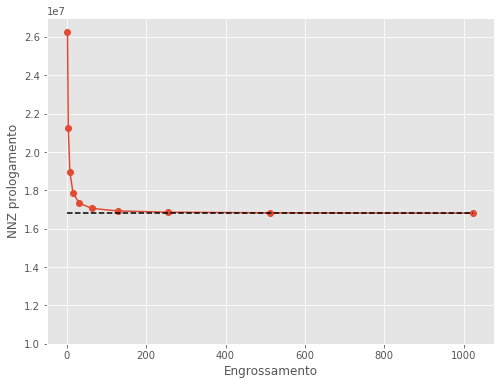
\includegraphics[width=8cm]{chap06/figs/nnzProlongamento.png}
\caption{Quantidade de não zeros do prolongamento $nnz_P$  em função do engrossamento da malha. A linha pontilhada mostra o valor de $16(n_x+1)(n_y+1)$.}
\label{fig:nnzGrafico}
\end{figure}
